\section{Auswertung}
\label{sec:Auswertung}

Die Graphen wurden sowohl mit Matplotlib \cite{matplotlib} als auch NumPy \cite{numpy} erstellt. Die Fehler werden mittels der Gauß´schen Fehlerfortpflanzung berechnet:
\begin{equation*}
\Delta f = \sqrt{\sum_{i=1}^n \left(\frac{\partial f}{\partial x_i}\Delta x_i\right)^2}
\end{equation*}
Dabei ist $f$ eine Größe, die von $n$ fehlerbehafteten Messgrößen $x_i$ abhängt.
Die Fehlerrechnung wurde mithilfe von Uncertainties \cite{uncertainties} durchgeführt.

\subsection{Approximation der Temperaturverläufe durch Polynome zweiten Grades}

Die Temperaturverläufe der beiden Wärmeresevoirs sind in Abbildung \ref{fig:Temperaturverläufe} dargestellt.
\noindent  Eine nichtlineare Ausgleichsrechnung der Form $y = At^2+Bt+C$ mittels SciPy \cite{scipy} liefert mit den Werten aus Tabelle \ref{tab:Messdaten} für das wärmere Reservoir folgende Parameter:
\begin{align*}
	A &= \SI{-2(1)e-7}{\kelvin\per\second\squared}\\
	B &= \SI{2.8(2)e-2}{\kelvin\per\second}\\
	C &= \SI{292.1(4)}{\kelvin}
\end{align*}
Für das kältere Reservoir ergibt sich entsprechend:
\begin{align*}
	A &= \SI{6(3)e-6}{\kelvin\per\second\squared}\\
	B &= \SI{-31(3)e-3}{\kelvin\per\second}\\
	C &= \SI{298.2(8)}{\kelvin}
\end{align*}
Die zugehörigen Graphen befinden sich in Abbildung \ref{fig:Temp1} und \ref{fig:Temp2}.
Für die Differentialquotienten $\frac{\text{d}T_1}{\text{d}t}$ und $\frac{\text{d}T_2}{\text{d}t}$ ergeben sich die Werte aus Tabelle \ref{tab:Ableitungen}.
\begin{table}
 	\centering
  	\caption{Die minütig aufgenommenen Messdaten}	
   	\label{tab:tabges}
	\sisetup{table-format=1.2}
	\begin{tabular}{S[table-format=2.1]S[table-format=2.1]S[table-format=1.2]S[table-format=2.2]S[table-format=3.0]}
		\toprule
		{$T_1 \si{\degreeCelsius}$} & {$T_2 \si{\degreeCelsius}$} & {$p_\text{a}/\si{\bar}$} & {$p_\text{b}/\si{\bar}$} & {$N_\text{mech}/\si{\watt}$} \\
		\midrule
		21.8 & 21.1 & 2.40 & 6.90 & 170 \\
		22.4 & 21.1 & 2.60 & 7.10 & 175 \\
		23.7 & 20.2 & 2.80 & 7.50 & 185 \\
		25.0 & 19.9 & 3.00 & 7.90 & 190 \\
		26.8 & 17.2 & 3.20 & 8.30 & 200 \\
		28.7 & 15.3 & 3.20 & 8.60 & 202 \\
		30.7 & 13.4 & 3.20 & 9.00 & 205 \\
		32.6 & 11.6 & 3.20 & 9.50 & 206 \\
		34.5 & 10.0 & 3.20 & 10.00 & 206 \\
		36.2 & 8.2 & 3.20 & 10.30 & 210 \\
		38.1 & 6.6 & 3.20 & 10.70 & 211 \\
		39.7 & 5.0 & 3.20 & 11.00 & 211 \\
		41.0 & 3.5 & 3.20 & 12.00 & 212 \\
		42.6 & 2.1 & 3.20 & 12.10 & 215 \\
		44.3 & 2.0 & 3.20 & 12.30 & 213 \\
		45.7 & 0.3 & 3.20 & 12.90 & 210 \\
		47.6 & -0.2 & 3.20 & 13.20 & 210 \\
		49.1 & -0.6 & 3.20 & 13.80 & 210 \\
		\bottomrule
	\end{tabular}
\label{tab:Messdaten}
\end{table}
\begin{figure}
	\centering
	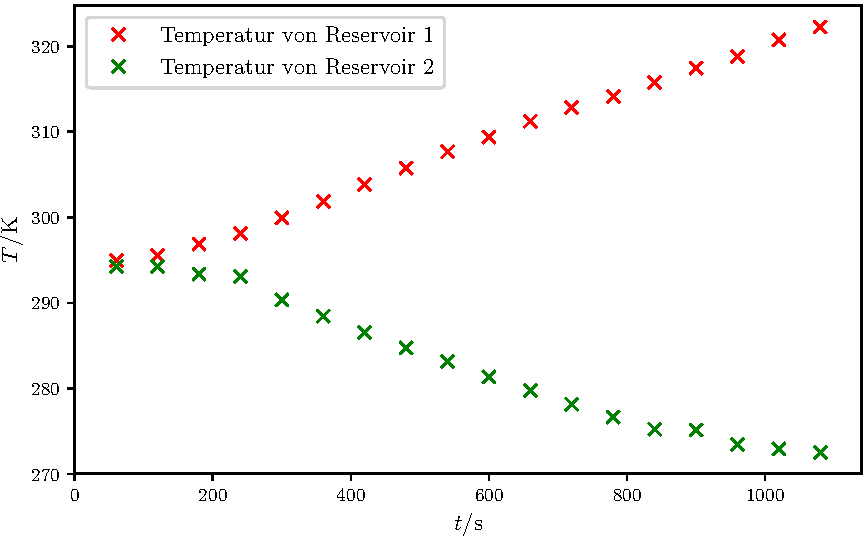
\includegraphics[scale = 1,keepaspectratio]
	{content/images/Temperaturen.pdf}
	\caption{Die Temperaturverläufe der Wärmeresevoirs}
	\label{fig:Temperaturverläufe}
\end{figure}
\begin{figure}
	\centering
	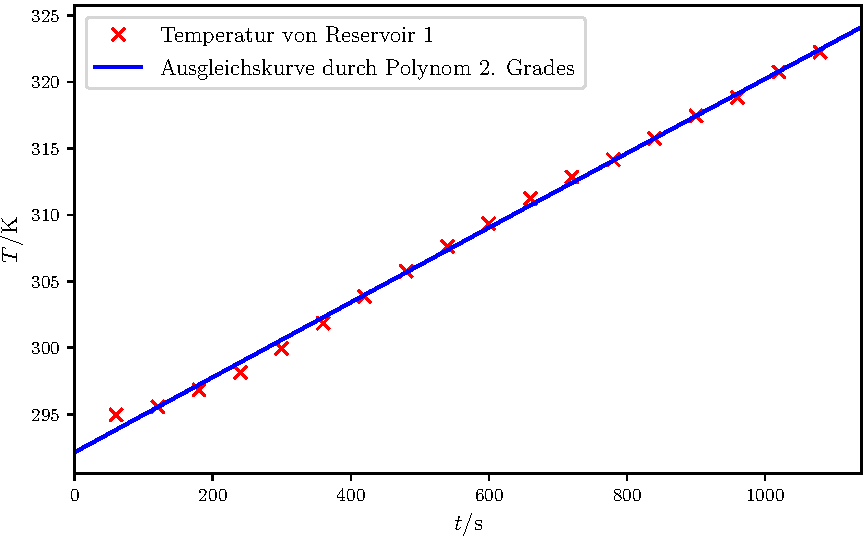
\includegraphics[scale = 1,keepaspectratio]
	{content/images/T1.pdf}
	\caption{Der Temperaturverlauf im wärmeren Reservoir mit Approximation }
	\label{fig:Temp1}
\end{figure}
\begin{figure}
	\centering
	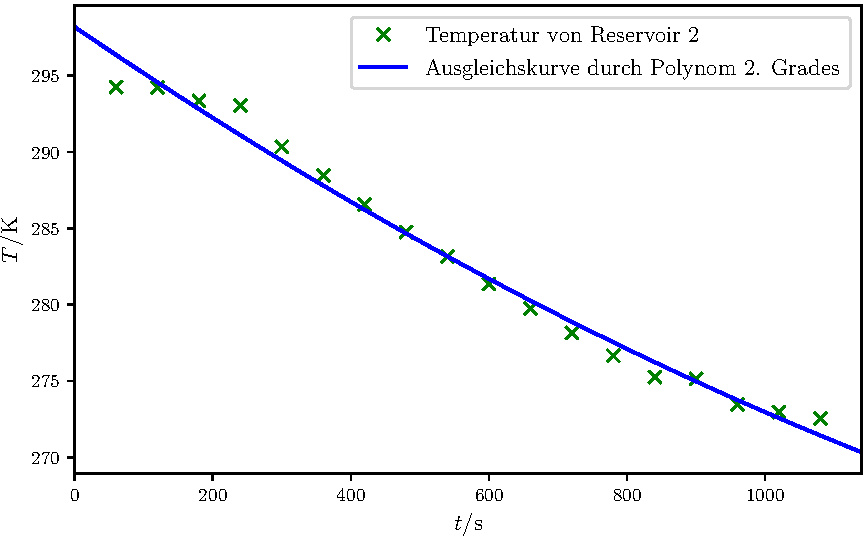
\includegraphics[scale = 1,keepaspectratio]
	{content/images/T2.pdf}
	\caption{Der Temperaturverlauf im kälteren Reservoir mit Approximation }
	\label{fig:Temp2}
\end{figure}
\begin{table}
  	\centering
  	\caption{Die Differenzenquotienten $\frac{\text{d}T_1}{\text{d}t}$ und $\frac{\text{d}T_2}{\text{d}t}$ zu 4 verschiedenen Zeiten.}
  	\label{tab:taba}
	\sisetup{table-format=1.2}
	\begin{tabular}{S[table-format=1.1]S[table-format=1.2]S[table-format=1.2]}
		\toprule
		{$r/\si{\centi\metre}$} & {$I/\si[per-mode=reciprocal]{\ampere}$} & {$B/\si[per-mode=reciprocal]{\milli\tesla}$} \\
		\midrule
		4.6 & 1.25 & 1.70 \\
		5.1 & 1.39 & 1.88 \\
		5.6 & 1.49 & 2.02 \\
		6.1 & 1.61 & 2.18 \\
		6.6 & 1.71 & 2.32 \\
		7.1 & 1.81 & 2.45 \\
		7.6 & 1.95 & 2.64 \\
		8.1 & 2.09 & 2.83 \\
		8.6 & 2.19 & 2.97 \\
		9.1 & 2.29 & 3.11 \\
		\bottomrule
	\end{tabular}
\label{tab:Ableitungen}
\end{table}

\subsection{Bestimmung der Güteziffer der Wärmepumpe und des Massendurchsatzes von Dichlordifluormethan }

Die Güteziffer der Wärmepumpe wird nach den Formeln \eqref{eq:Q2/dt} und \eqref{eq:ny} berechnet. Die ideale Güte folgt aus Formel \eqref{eq:nyideal}. 
Dabei besitzt das Wasser eine spezifische Wärmekapazität von $c_.W=\SI{4.18}{\joule\per\gram\per\kelvin}$\cite{V201}. Die Apparatur hat nach Angabe eine Wärmekapazität von $\SI{660}{\joule\per\kelvin}$. In den Wärmereservoirs befindet sich jeweils eine Wassermenge von drei Litern. Mithilfe der zuvor bestimmten vier Temperaturen ergeben sich die Werte aus Tabelle \ref{tab:Güte}. 
\begin{table}
	\centering
	\caption{Die reale Güte der Wärmepumpe zu vier Zeiten und der zugehörige ideale Wert}
 	\label{tab:tabv}
	\sisetup{table-format=1.2}
	\begin{tabular}{S[table-format=3.0]S[table-format=1.1] @{${}\pm{}$} S[table-format=1.1]S[table-format=2.1]}
		\toprule
		{t/\si{\second}} & \multicolumn{2}{c}{$v_\text{real}$} & {$v_\text{ideal}$} \\
		\midrule
		240 & 1.9 & 0.1 & 31.2 \\
		480 & 1.8 & 0.1 & 12.6 \\
		720 & 1.7 & 0.2 & 8.4 \\
		960 & 1.8 & 0.2 & 6.7 \\
		\bottomrule
	\end{tabular}
\label{tab:Güte}
\end{table}
\newline
\noindent Um den Massendurchsatz von Dichlordifluormethan bestimmen zu können, muss die Verdampfungswärme des Transportgases bestimmt werden. Es gilt:
\begin{align*}
 	 L &= -\ln\left(\frac{p}{p_0}\right) RT\\
	    &= - A R
\end{align*}
Dabei ist $p_0 = \SI{1}{\bar}$ und A ist die Steigung des Graphen, wenn $\ln\left(\frac{p}{p_0}\right)$ gegen $1/T$ aufgetragen wird. Sie kann durch eine lineare Ausgleichsrechnung ermittelt werden. $R = \SI{8.314}{\joule\per\mol\per\kelvin}$ \cite{R} ist die allgemeine Gaskonstante.
Mit $p=p_.b$ und $T=T_.1$ folgt:
\begin{align*}
 	 L = \SI{1.94(4)e+4}{\joule\per\mol}\text{.}
\end{align*}
\begin{figure}
 	\centering
 	\caption{Der Verlauf der Dampfdruckkurve von Dichlordifluormethan in Abhängigkeit der reziproken Temperatur.}
 	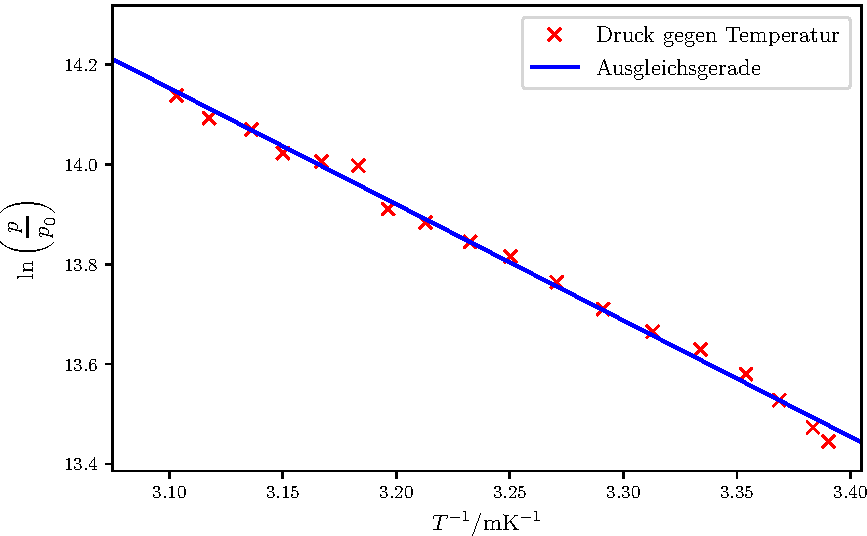
\includegraphics[width=\linewidth-70pt,height=\textheight-70pt,keepaspectratio]{content/images/Dampfdruck.pdf}
 	\label{fig:Dampfdruck}
\end{figure}
\newline
\noindent Mit Formel \eqref{eq:Md2} ergibt sich der Massendurchsatz aus Tabelle \ref{tab:Massendurchsatz}.
 \begin{table}
   	\centering
   	\caption{Der bestimmte Massendurchsatz zu 4 verschiedenen Zeitpunkten.}
   	\label{tab:tabm}
	\sisetup{table-format=1.2}
	\begin{tabular}{S[table-format=3.0]S[table-format=1.2] @{${}\pm{}$} S[table-format=1.2]}
		\toprule
		{t/\si{\second}} & \multicolumn{2}{c}{$\frac{\text{d}m}{\text{d}t}/\si[per-mode=reciprocal]{\gram\per\second}$} \\
		\midrule
		240 & 0.35 & 0.03 \\
		480 & 0.31 & 0.04 \\
		720 & 0.28 & 0.05 \\
		960 & 0.25 & 0.07 \\
		\bottomrule
	\end{tabular}
\label{tab:Massendurchsatz}
 \end{table}

\subsection{Bestimmung der Leistung des Kompressors}

Die Leistung des Kompressors lässt sich nach den Formeln \eqref{eq:P} und \eqref{eq:rho} bestimmen. Mit einem $\rho_0 = \SI{5.51}{\gram\per\litre}$ \cite{V206}, einer Normaltemperatur $T_0 = \SI{273.15}{\kelvin}$,  einem Normaldruck $p_0 = \SI{1}{\bar}$ und einem $\kappa = 1.44$ \cite{V206} ergeben sich die Leistungen in Tabelle \ref{tab:tabn}.

 \begin{table}
  \centering
  \caption{Die bestimmte Leistung zu 4 verschiedenen Zeitpunkten.}
  \label{tab:tabn}
	\sisetup{table-format=1.2}
	\begin{tabular}{S[table-format=3.1]S[table-format=3.1]S[table-format=3.1]S[table-format=2.1]S[table-format=1.2]@{${}\pm{}$}S[table-format=1.5]}
		\toprule
		{$\lambda/10^{-9}\si{\metre}$} & {$\Omega_.r/\si{\degree}$} & {$\Omega_.l/\si{\degree}$} & {$\eta/\si{\degree}$} &  \multicolumn{2}{c}{$n$} \\
		\midrule
		404.7 & 215.3 & 105.0 & 69.7 & 1.81 & 0.00056 \\
		407.8 & 215.4 & 104.9 & 69.5 & 1.81 & 0.00056 \\
		435.8 & 216.3 & 104.0 & 67.7 & 1.80 & 0.00055 \\
		480.0 & 217.2 & 103.2 & 66.0 & 1.78 & 0.00054 \\
		491.6 & 217.3 & 102.9 & 65.6 & 1.78 & 0.00053 \\
		508.6 & 217.8 & 102.4 & 64.6 & 1.77 & 0.00053 \\
		546.1 & 218.2 & 102.0 & 63.8 & 1.76 & 0.00052 \\
		577.0 & 218.5 & 101.7 & 63.2 & 1.76 & 0.00052 \\
		579.1 & 218.6 & 101.6 & 63.0 & 1.76 & 0.00052 \\
		643.8 & 219.2 & 101.1 & 61.9 & 1.75 & 0.00051 \\
		\bottomrule
	\end{tabular}
\label{tab:Leistung}
\end{table}
